\documentclass[12pt]{article}
\usepackage{geometry}                % See geometry.pdf to learn the layout options. There are lots.
\geometry{letterpaper}                   % ... or a4paper or a5paper or ... 
%\geometry{landscape}                % Activate for for rotated page geometry
\usepackage[parfill]{parskip}    % Activate to begin paragraphs with an empty line rather than an indent
\usepackage{./styles/daves,fancyhdr,natbib,graphicx,dcolumn,amsmath,lastpage,url}
\usepackage{amsmath,amssymb,epstopdf,longtable}
\usepackage[final]{pdfpages}
\DeclareGraphicsRule{.tif}{png}{.png}{`convert #1 `dirname #1`/`basename #1 .tif`.png}
\pagestyle{fancy}
\lhead{CE 5362 -- Surface WaterModeling}
\rhead{SPRING 2020}
\lfoot{}
\cfoot{}
\rfoot{Page \thepage\ of \pageref{LastPage}}
\renewcommand\headrulewidth{0pt}



\begin{document}
\begin{center}
{\textbf{{ CE 5362 Surface Water Modeling} \\ {Project 4}}}
\end{center}

\section*{{Problem Statement}}
Figure  \ref{fig:HoustonBase} is a Google Earth Image of the confluence of Buffalo and White Oak Bayou in Houston Texas.

\begin{figure}[h!] %  figure placement: here, top, bottom, or page
   \centering
   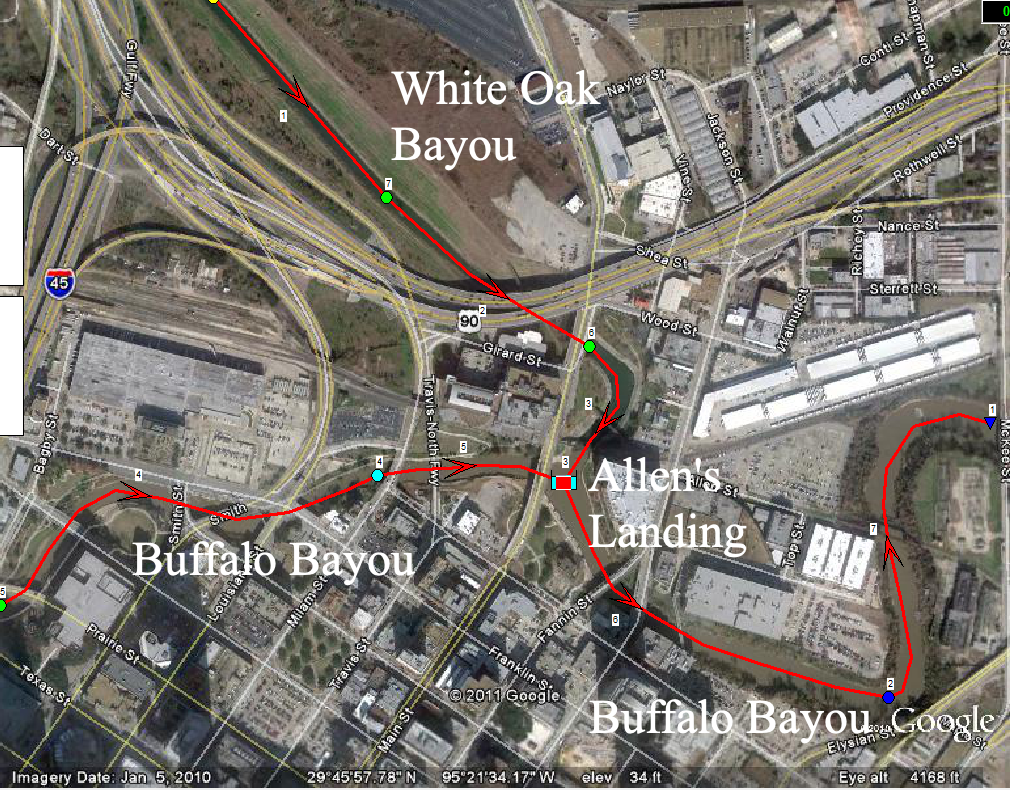
\includegraphics[width=5.5in]{HoustonBase.png} 
   \caption{Plan view/schematic for example}
   \label{fig:HoustonBase}
\end{figure}

\clearpage

Figure  \ref{fig:BuffaloDownstream} is a graphical representation of a cross section on Buffalo Bayou  about one mile downstream of Allen's Landing.


\begin{figure}[h!] %  figure placement: here, top, bottom, or page
   \centering
   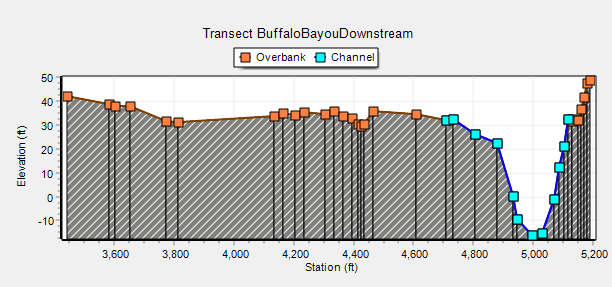
\includegraphics[width=5.5in]{BuffaloDownstream.png} 
   \caption{Cross section, Buffalo Bayou Downstream 4340 feet from Allen's Landing}
   \label{fig:BuffaloDownstream}
\end{figure}
Tabular values of cross section survey elevations and Manning's n values are shown below.
\begin{verbatim}
# buffalo bayou downstream
# about 4340 feet downstream of confluence
STATION  ELEVATION  MANNING_N
3444.4	42.1	0.15
3584.4	38.8	
3604.4	38.1	
3654.4	38.1	
3774.4	31.9	
3814.4	31.4	
4134.4	34	
4164.4	35.2	
4204.4	34.3	
4234.4	35.3	
4304.4	34.8	
4334.4	35.9	
4364.4	33.6	
4394.4	33	
4414.4	30.3	
4424.4	29.6	
4434.4	30.3	
4464.4	35.9	
4608.8	34.6	
4708.8	32	
4730.2	32.62	0.035
4806.4	26.29	
4879.1	22.6	
4930.6	0.07	
4945.8	-9.41	
4996	-16.14	
5029.6	-15.3	
5069.5	-0.94	
5086.1	12.41	
5102.5	21.32	
5116.8	32.62	0.2
5127.1	32.34	
5128.8	31.8	
5148.8	32.2	
5158.8	36.6	
5168.8	41.7	
5178.8	47.5	
5188.8	48.9	
\end{verbatim}


Figure  \ref{fig:BuffaloUpstream} is a graphical representation of a cross section on Buffalo Bayou about one mile upstream of Allen's Landing..
\begin{figure}[h!] %  figure placement: here, top, bottom, or page
   \centering
   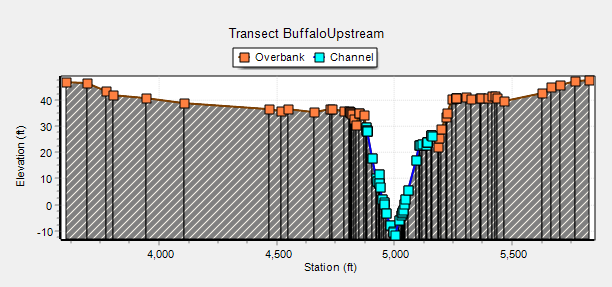
\includegraphics[width=5.5in]{BuffaloUpstream.png} 
   \caption{Cross section, Buffalo Bayou Upstream 4087 feet from Allen's Landing}
   \label{fig:BuffaloUpstream}
\end{figure}

Tabular values of cross section survey elevations and Manning's n values are shown below.
\begin{verbatim}
# buffalo upstream
# near allen parkway
# approx. 4087 feet upstream of confluence
STATION ELEVATION MANNING_N
3604.2	46.74	0.2
3694.2	46.24	
3774.2	43.24	
3804.2	41.64	
3944.2	40.44	
4106.5	38.64	
4467.3	36.54	
4517.3	35.74	
4547.3	36.24	
4657.3	35.14	
4727.3	36.54	
4737.1	36.42	
4786	35.81	
4807.3	35.54	
4812.69	35.16	
4812.8	35.16	
4812.91	35.15	
4817.3	34.84	
4818.7	34.54	
4828.7	32.74	
4838.7	30.14	
4851.7	34.79	
4851.8	34.78	
4869.2	33.99	
4879.4	29.42	0.07
4881.9	28.29	
4882	28.25	
4882.11	28.2	
4882.2	28.16	
4905.3	17.8	
4921.7	10.01	
4926	8.95	
4926.1	8.93	
4933.4	8.3	
4933.7	11.5	
4934.6	8.13	0.04
4937.4	6.84	
4947.4	2.25	
4956	1.17	
4957.9	0.35	
4965.2	-3	
4983.3	-7.73	
4992.6	-9.93	
4996.3	-10.52	
5002.5	-11.52	
5020.1	-5.95	
5027.5	-3.96	
5032	-2.98	
5032.2	-2.92	
5035.5	-1.94	
5042	0.34	
5046.9	2.14	
5056.7	5.42	
5090.6	17.19	
5106	22.54	0.07
5108.9	22.71	
5119.5	23.01	
5133	22.72	
5138.4	23.7	
5139.79	23.95	
5139.9	23.97	
5140.01	23.99	
5154.6	26.63	
5154.7	26.62	
5159.2	26	0.2
5187.6	22.14	
5188.7	25.44	
5198.7	28.64	
5218.7	33.54	
5225	34.74	
5245	40.24	
5261.2	40.43	
5261.29	40.43	
5261.4	40.43	
5261.5	40.43	
5305	40.94	
5326.9	40.34	
5365.9	40.73	
5366.9	40.74	
5396.9	40.74	
5416.9	41.54	
5426.9	41.44	
5436.8	40.44	
5466.8	39.54	
5626.8	42.34	
5666.8	44.74	
5706.8	45.64	
5768	47.24	
5828	47.44	
\end{verbatim}


Figure  \ref{fig:WhiteOakUpstraeam} is a graphical representation of a cross section on White Oak Bayou about one mile upstream of Allen's Landing..
\begin{figure}[h!] %  figure placement: here, top, bottom, or page
   \centering
   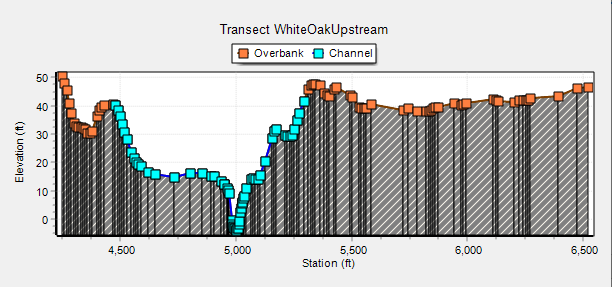
\includegraphics[width=5.5in]{WhiteOakUpstraeam.png} 
   \caption{Cross section, White Oak Bayou Upstream 6602 feet from Allen's Landing}
   \label{fig:WhiteOakUpstraeam}
\end{figure}

Tabular values of cross section survey elevations and Manning's n values are shown below.
\begin{verbatim}
# WhiteOakBayou I-45 N Ramp 
# cross section 4
# approx 6602 feet upstream of confluence
STATION  ELEVATION  MANNING_N  
4247.7	50.48	0.05
4257.7	48.13	
4267.7	45.44	
4277.7	41.1	
4287.7	37.37	
4297.7	33.89	
4307.7	32.78	
4317.7	32.5	
4327.7	32.54	
4337.7	32.25	
4347.7	31.64	
4357.7	30.49	
4367.7	30.32	
4377.7	31.14	
4397.7	36.41	
4407.7	38.57	
4417.7	39.65	
4427.7	40.3	
4467.7	40.71	
4477.7	40.4	
4487.7	38.43	
4497.7	36.25	
4507.7	33.65	
4517.7	30.79	
4527.7	28.18	
4547.7	23.55	
4557.7	21.52	
4567.7	20.14	
4577.7	19.23	
4587.7	18.82	
4617.7	16.53	
4651.6	15.86	
4731.6	14.61	
4801.6	16.1	
4851.6	16.11	
4893.6	15.17	
4903.6	15.01	
4935.3	13.21	
4947.51	12.24	
4949.28	12.14	
4960.01	10.77	0.015
4963.39	10.2	
4967.88	9.07	
4982.44	-0.3	
4984.71	-1.72	
4986.11	-2.47	
4987.24	-2.94	
4992.7	-3.18	
4993.75	-3.3	
5000	-4.3	
5000.86	-4.1	
5001.13	-3.99	
5003.39	-3.29	
5008.5	-3.11	
5010.89	-1.91	
5013.03	-0.74	
5019.05	2.47	
5021.77	3.92	
5025.43	5.69	
5026.05	5.79	
5032	7.19	
5035.85	8.14	
5043.6	10.81	0.05
5063.6	13.97	
5073.6	14.42	
5083.6	14.17	
5093.6	14.2	
5103.6	15.48	
5123.6	20.42	
5153.6	28.69	
5163.6	30.96	
5173.6	31.69	
5212.4	29.67	
5222.4	29.3	
5232.4	29.16	
5242.4	29.62	
5252.4	31.89	
5262.4	35.02	
5272.4	37.34	
5292.4	41.72	
5312.4	45.74	
5322.4	47.16	
5332.4	47.59	
5342.4	47.75	
5362.4	47.28	
5382.4	44.52	
5392.4	43.7	
5402.4	43.35	
5422.4	45.98	
5432.4	46.48	
5492.4	43.71	
5502.4	43.02	
5532.4	39.7	
5542.4	39.06	
5552.4	39.08	
5562.4	39.32	
5582.4	40.47	0.99
5722.4	38.58	
5742.4	39.05	
5782.4	38.24	
5822.4	38.03	
5832.4	38.19	
5842.4	38.61	
5852.4	39.29	
5862.4	39.5	
5872.4	39.41	
5942.4	40.78	
5972.4	40.39	
5982.4	40.47	
5992.4	40.98	
6112.4	42.24	
6122.4	42.13	
6132.4	41.71	
6202.4	41.44	
6222.4	42.09	
6242.4	42.14	
6252.4	41.96	
6262.4	42.11	
6272.4	42.53	
6392.4	43.41	
6472.4	46.12	
6521.7	46.47	
\end{verbatim}

Bottom elevations near the confluence are:
\begin{itemize}
\item White Oak, just upstream of confluence = - 6.71 ft
\item Buffalo Bayou, just upstream of confluence = - 9.31 ft
\item Buffalo Bayou, just downstream of confluence = - 14.28 ft
\end{itemize}

The confluence dimensions at low flow (2000 cfs) are roughly 80 feet across Buffalo Bayou,and 120 feet across White Oak.

The angle between White Oak and Buffalo downstream is 38-degrees, and the angle between White Oak and Buffalo upstream is 70-degrees.

The three cross sections above have the following additional relationships

Distance from junction to Buffalo Bayou Upstream cross section = 4087 feet.\\
Distance from junction to Buffalo bayou Downstream cross section = 4340 feet.\\
Distance from junction to White Oak Bayou upstream cross section = 6602 feet.\\

\begin{tabular}{p{1.5in}p{0.9in}p{0.8in}p{1.65in}p{1in}}
Cross Section Name & Low Elev.&Distance& Delta Z&Slope \\
\hline
\hline
White Oak Upstream & -4.3 feet & 6602 feet & (-4.3)-(-6.71) = 2.41& So=  0.03\% \\
Buffalo Upstream & -11.52 feet & 4087 feet & (-11.52)-(-9.31) =-2.21 &So= -0.054\% (adverse) \\
Buffalo Downstream &  -16.14 feet &4340 feet & (-14.28)-(-16.14)= 1.86 &So=  0.042\% \\
\hline
\end{tabular}

Rating curves for the various cross sections are presented in the supporting files.

Using the hydrographs in the following document simulate the behavior of the confluence is steady (peaks at same time) and dynamic conditions.
Produce a plot of the water depth in the confluence under these two conditions.

Discuss how you choose to model the downstream boundary conditions.



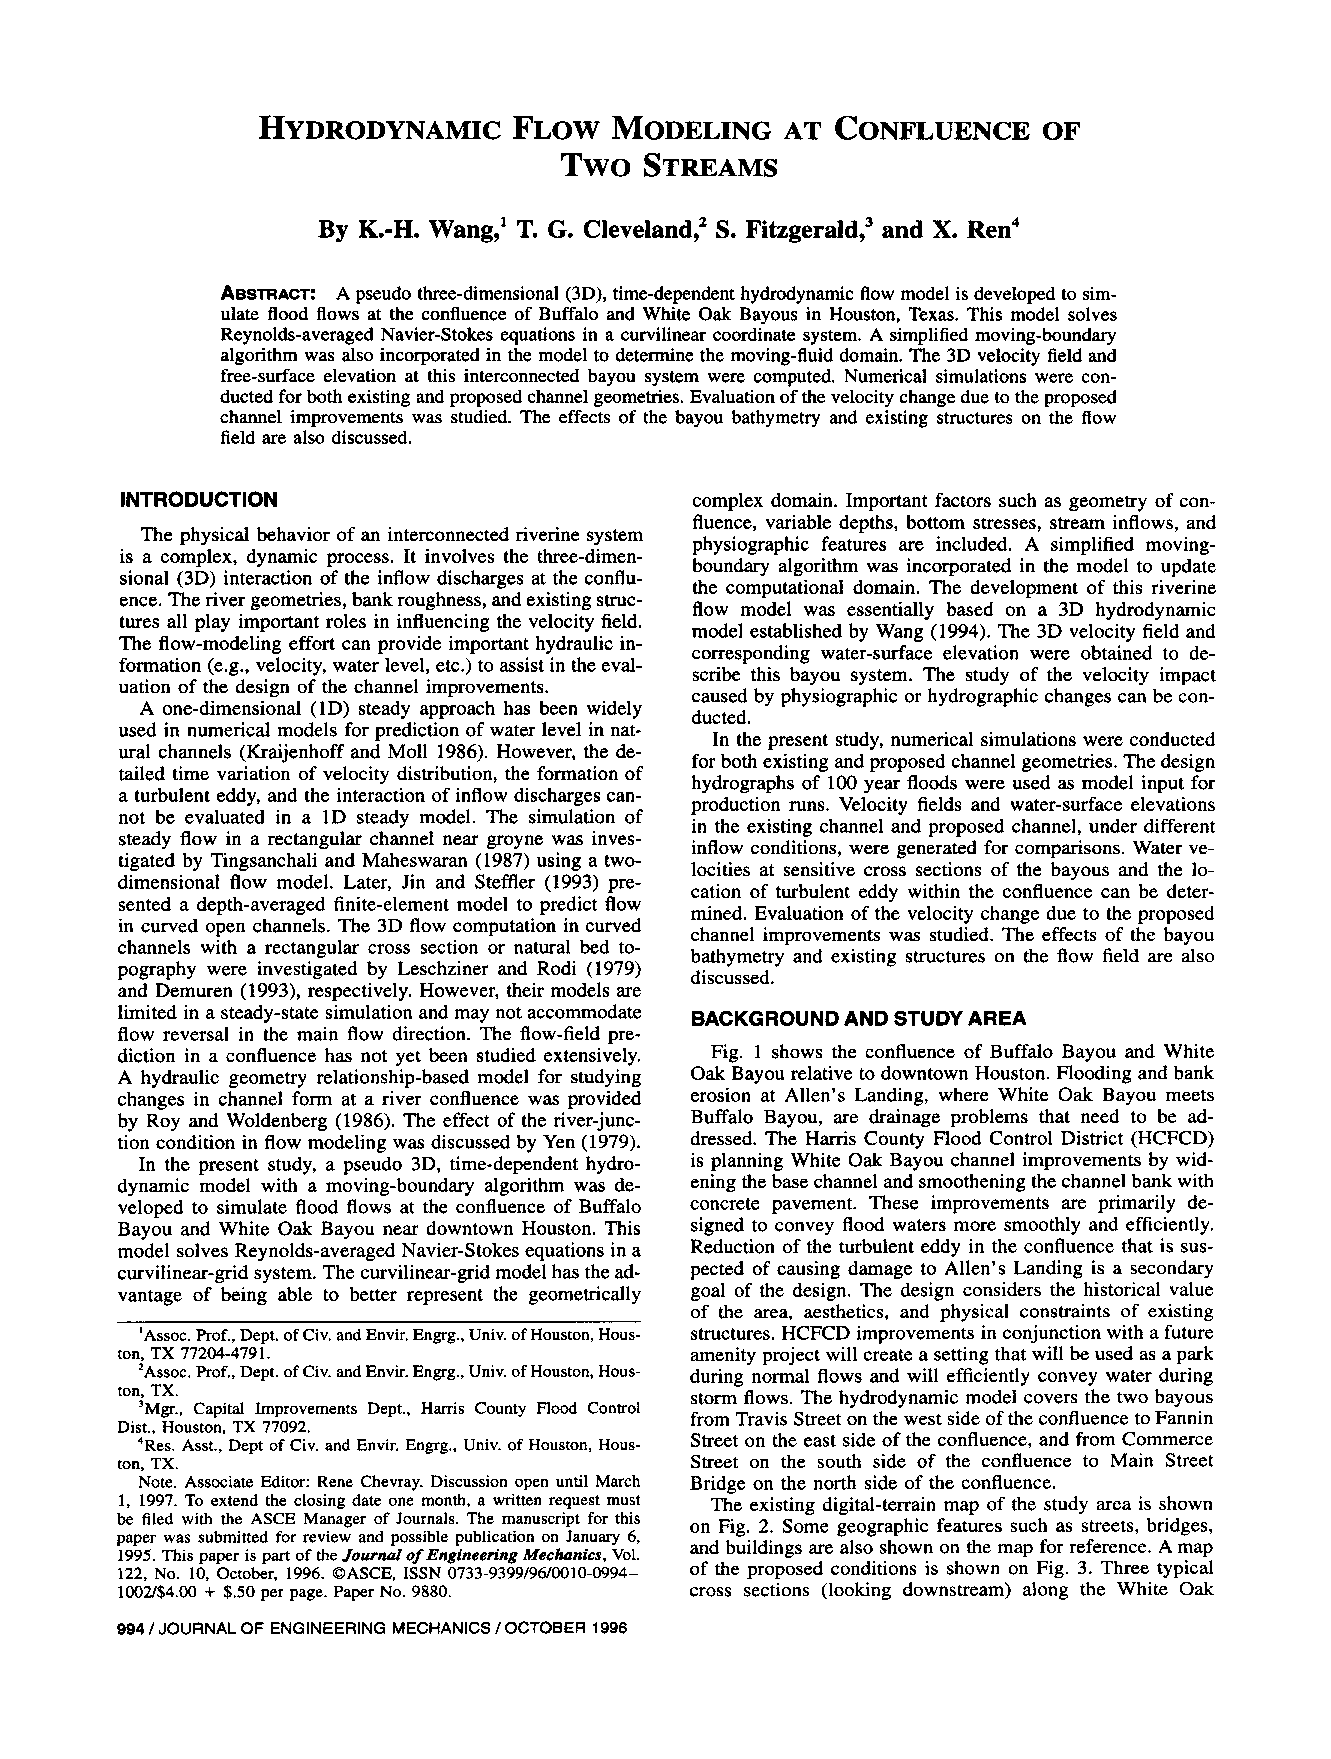
\includepdf[pages={-}]{HydrodynamicFlowModeling.pdf}\end{document} p{2in} 